\chapter{Service Cutter Assessment}
\label{testSystems}

We used two example systems to test the Service Cutter. After defining the input used to describe the systems we discussed and documented our expectations on how service decomposition of the systems would make sense from our experience. In order to rate the candidate service cuts provided by the service cutter we defined three categories of cuts:

\begin{description}
	\item[Expected Service Cut] The cut is exactly the way we expected it. 
	\item[Reasonable Service Cut] The cut is not the way we expected it but we find reasons why the cut could make sense from an architects perspective.
	\item[Unreasonable Service Cut] The cut is not as we expected it and we do not find reasons why the cut would provide any benefits to a systems architecture. 
\end{description}

To assess the Service Cutter's output the following language is used:

\begin{itemize}
	\item An \textit{good} output contains zero unreasonable service cuts.
	\item An \textit{acceptable} output contains at most one unreasonable service cut.
	\item A \textit{bad} output contains two or more unreasonable service cuts.
\end{itemize}


\section{Trading System}
\label{sec:tradingSystem}

We developed the Trading System as a fictional example based on personal experience with similar systems. Its goal is to include various different coupling aspects in a rather small model.

The Trading System is an application one might find in a typical swiss private bank offering its customers the ability to manage their stocks portfolio.

\begin{itemize}
\item The main focus is to buy or sell \textit{stocks} at a specific price (\textit{Order.triggerPrice}) using an \textit{order}.
\item \textit{Prices} are frequently imported from a market data provider and upon import of a price, all orders are checked for orders that can be triggered.
\item When an order is executed, an instruction is sent to the market to purchase or sell the stocks. The \textit{PaymentInfo} contains all necessary information to do so. 
\item \textit{News} are imported from an external provider and are linked to a specific stock. They provide valuable, contextual information when using the system. However traders and customers can easily fall back to any online source should this information not be available.
\item \textit{Recommendations} are suggested to the user of the system based on his existing portfolio.
\end{itemize}

Figure \ref{fig:tradingClasses} shows a domain model of the Trading System.

\begin{figure}[H]
	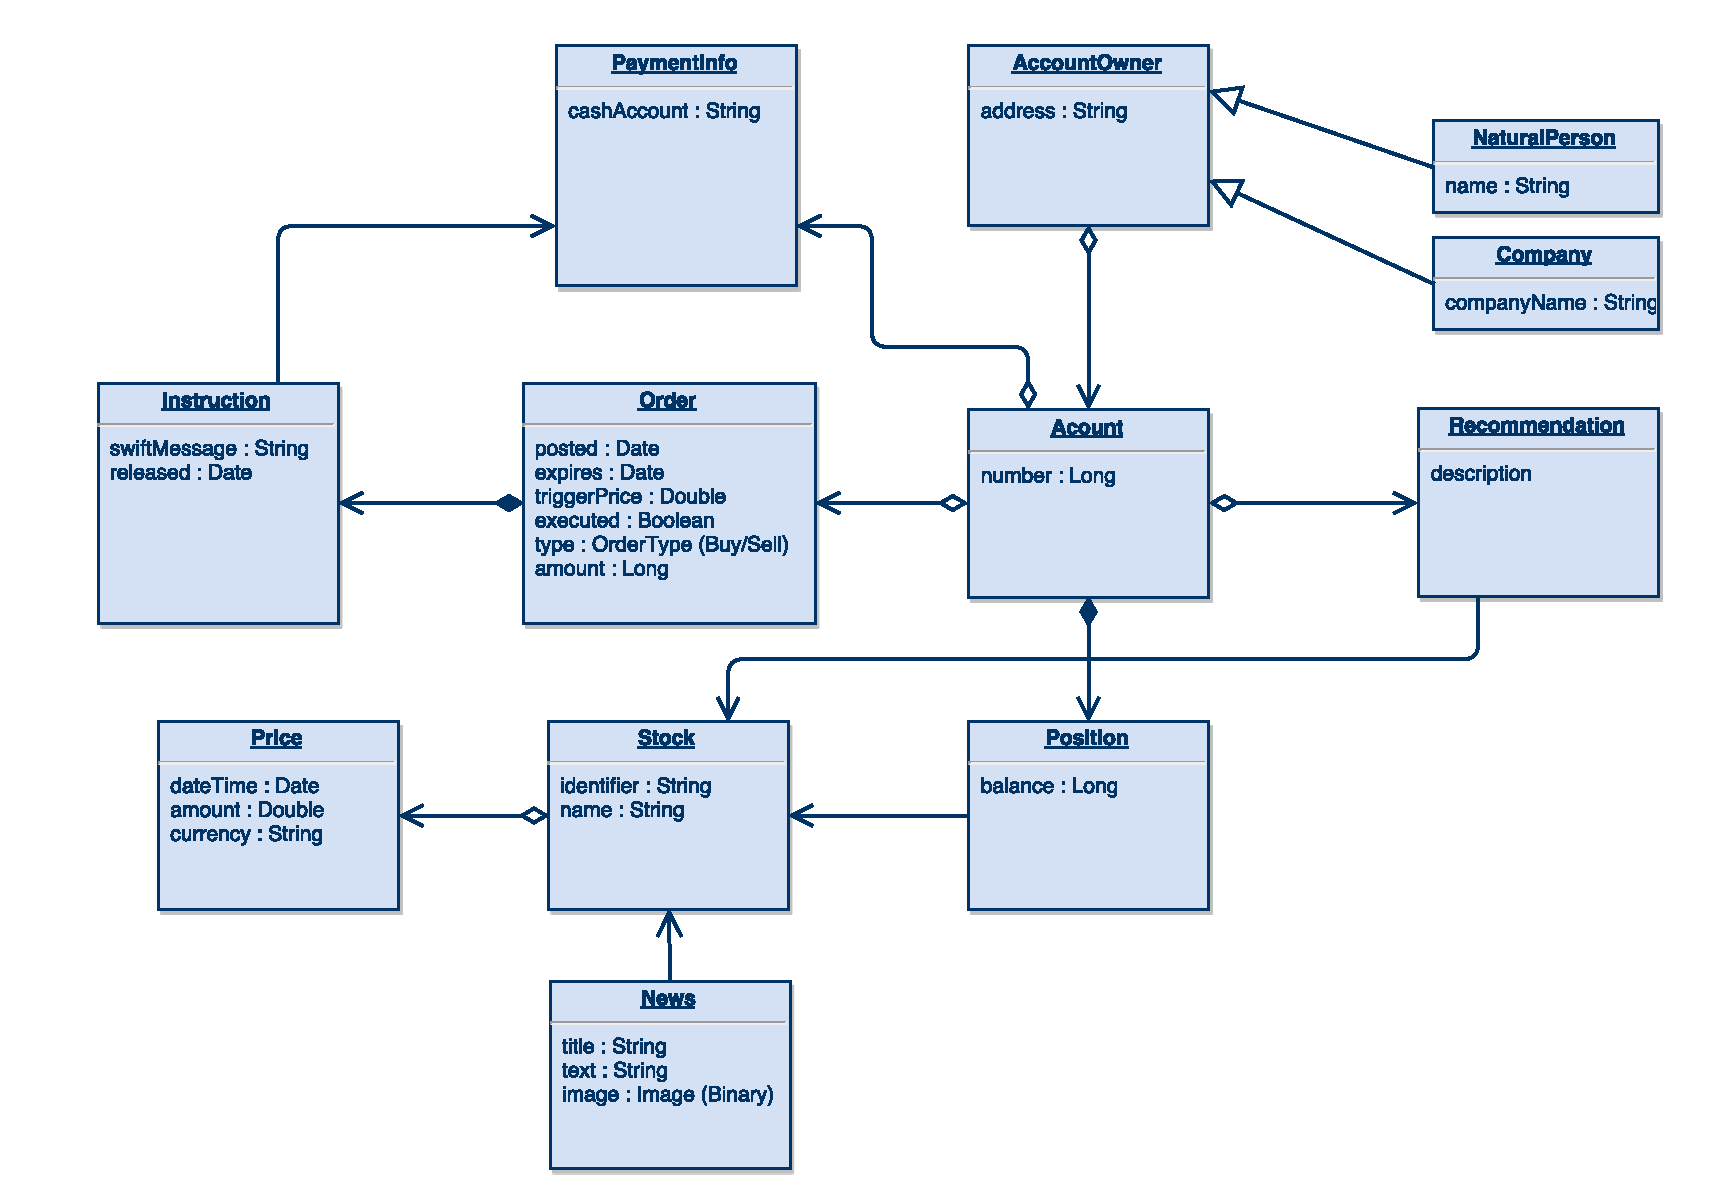
\includegraphics[scale=0.5]{diagrams/TradingSystem.pdf}
	\caption{Trading System Class Diagram}
	\label{fig:tradingClasses}
\end{figure}

The following ten use cases describe the supported functionality of the application.

\begin{enumerate}
\item Post Order
	\begin{itemize}
	\item Nanoentities written: Order.posted,  Order.expires, Order.triggerPrice, Order.executed, Order.type, Order.amount
	\item Nanoentities read: Account.number, Stock.identifier, Stock.stockName
	\end{itemize}
\item Instruct Order
	\begin{itemize}
	\item Nanoentities written: Instruction.instructedTime, Order.executed, Position.balance
	\item Nanoentities read: PaymentInfo.cashAccount
	\end{itemize}
\item Import Price and Check for Due Orders (Technical)
	\begin{itemize}
	\item Nanoentities written: Price.dateTime, Price.price, Price.currency
	\item Nanoentitiess read: Order.triggerPrice, Stock.identifier
	\end{itemize}
\item Read News
	\begin{itemize}
	\item Nanoentities written: - 
	\item Nanoentities read: Stock.identifier, News.title, News.text, News.image
	\end{itemize}
\item Import News (Technical)
	\begin{itemize}
	\item Nanoentities written: News.title, News.text, News.image
	\item Nanoentities read: Stock.identifier
	\end{itemize}
\item View Recommendations
	\begin{itemize}
	\item Nanoentities written: -
	\item Nanoentities read: Account.number, Recommendation.description, Stock.identifier, Stock.stockName
	\end{itemize}
\item Suggest Recommendations (Technical)
	\begin{itemize}
	\item Nanoentities written: Recommendation.description
	\item Nanoentities read: Account.number, Stock.identifier, Stock.stockName, Position.balance
	\end{itemize}
\item Create Account
	\begin{itemize}
	\item Nanoentities written: Account.number
	\item Nanoentities read: AccountOwner.address, NaturalPerson.name, Company.companyName
	\end{itemize}
\item Create Account Owner
	\begin{itemize}
	\item Nanoentities written: AccountOwner.address, NaturalPerson.name, Company.companyName
	\item Nanoentities read: -
	\end{itemize}
\item View Portfolio
	\begin{itemize}
	\item Nanoentities written: -
	\item Nanoentities read: Account.number, Position.balance, Stock.identifier, Stock.stockName, Order.triggerPrice, Order.amount, Order.posted, Order.expires, Order.executed, Order.type
	\end{itemize}
\end{enumerate}

In addition to the use cases, we defined the following characteristics.

\textbf{Security Criticality}

\begin{itemize}
\item \textbf{Critical}: AccountOwner.address, NaturalPerson.name, Company.companyName
\item \textbf{Public}: Stock.identifier,Stock.stockName, Price.dateTime, Price.price, Price.currency, News.title, News.text, News.image
\end{itemize} 

\textbf{Volatility}

\begin{itemize}
\item \textbf{Often}: Price.dateTime, Price.price, Price.currency
\item \textbf{Rarely}: AccountOwner.address, NaturalPerson.name, Company.companyName, Account.number
\end{itemize}

\textbf{Consistency}

\begin{itemize}
\item \textbf{Eventually}: Price.dateTime, Price.price, Price.currency
\end{itemize}

\textbf{Storage Similarity}

\begin{itemize}
\item \textbf{Huge}: News.image
\end{itemize}

\textbf{Change Similarity}

\begin{itemize}
\item \textbf{Often}: Recommendation.description
\end{itemize}

\textbf{Resilience}

\begin{itemize}
\item \textbf{Low}: News.title, News.text, News.image, Recommendation.description
\end{itemize}

Furthermore all default characteristics as documented in Section \ref{sec:couplingCriteria} are taken into account.

\subsection{Expected Service Cuts}

From our experience in software architecture we expect the Service Cutter to decompose the Trading System into the services presented in Figure \ref{fig:tradingCuts}.

\begin{figure}[H]
	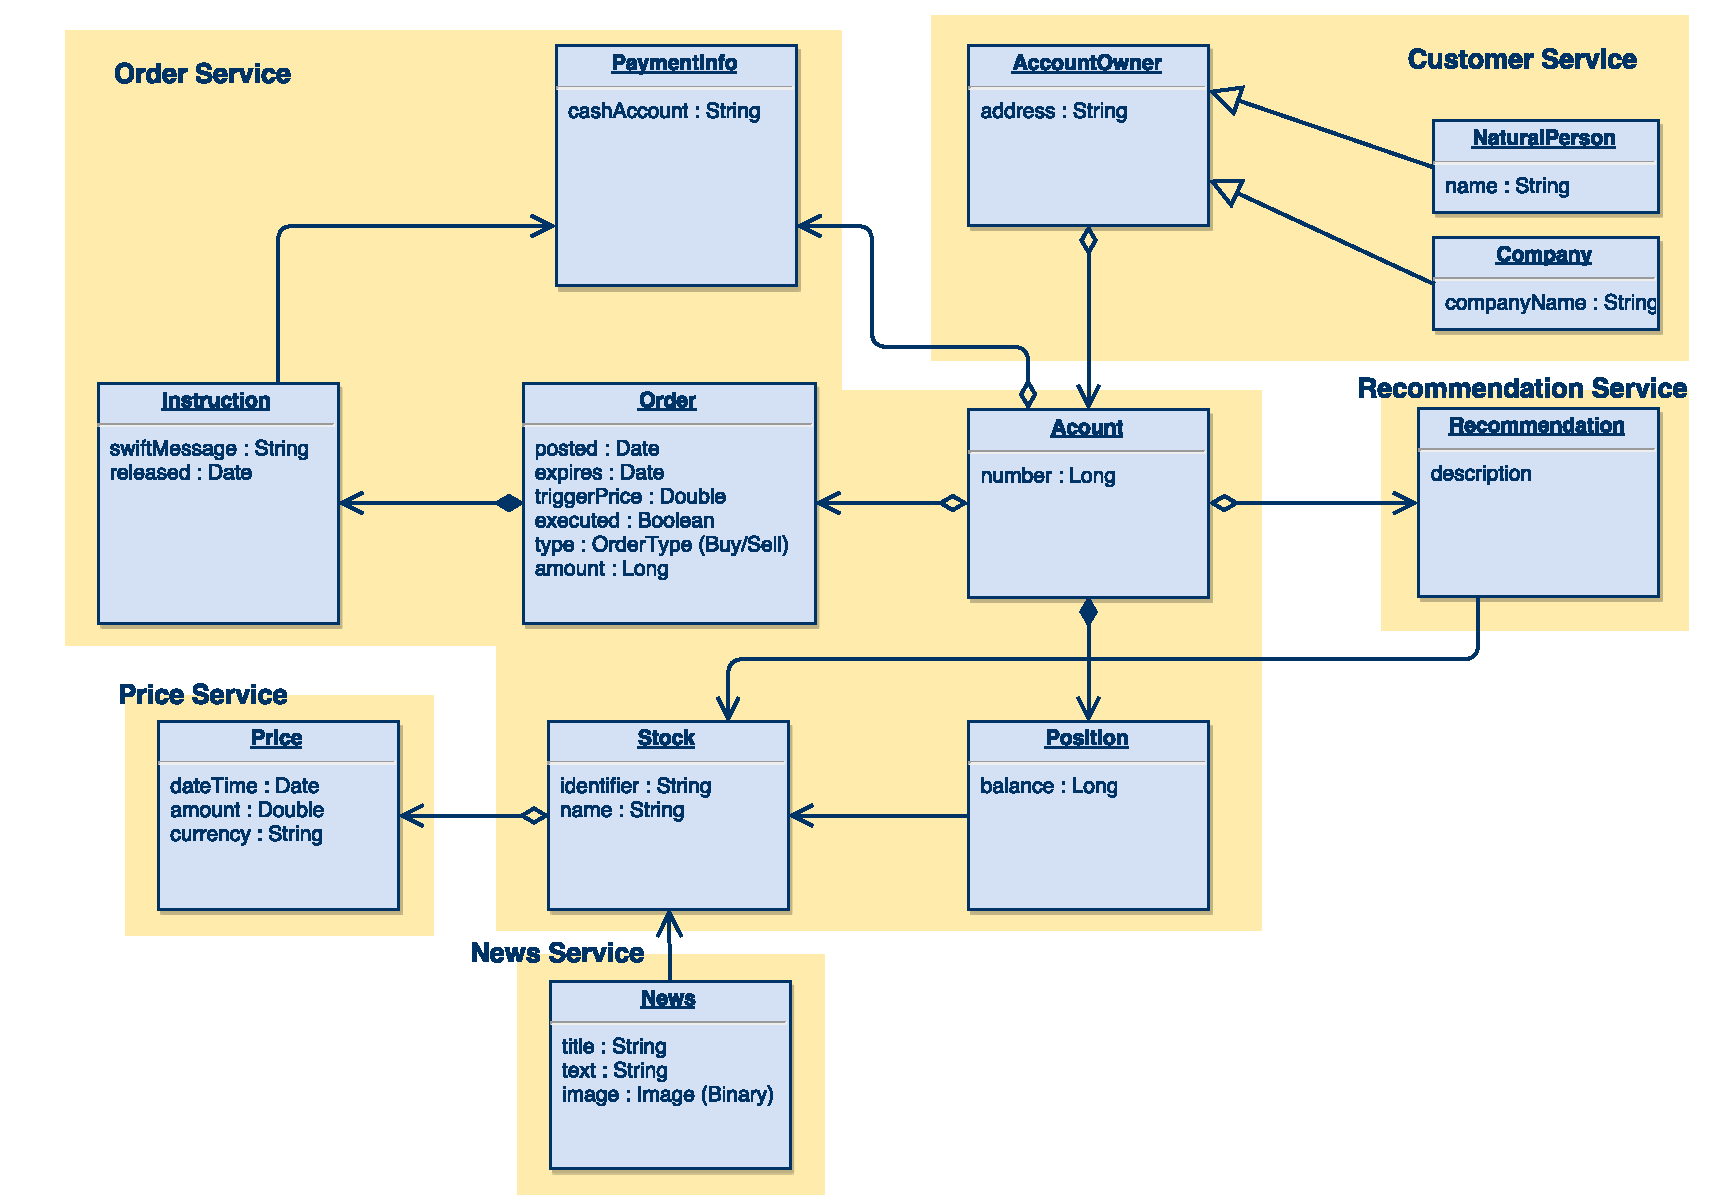
\includegraphics[scale=0.5]{diagrams/TradingSystem-ServiceCut.pdf}
	\caption{Trading System expected service cuts}
	\label{fig:tradingCuts}
\end{figure}

The following reasons led us to this decision.
\begin{itemize}
	\item The service \textit{Order} encapsulates many use cases and contains several entities that need to be processed with high consistency (Order, Position).
	\item The high volatility of the entity price led to the isolation of this part into an own service \textit{Price}.
	\item News are not part of the core operations and therefore require lower resilience and security criticality. News images furthermore require a significant amount of storage. Therefore we would isolate this into a separate \textit{News} service.
	\item The recommendation algorithm will be changed frequently. A dedicated \textit{Recommendation} service allows independent deployment of updated versions. Moreover recommendations are, like the news, not part of the core operations and require lower resilience. 
	\item Security restrictions requires all \gls{PII} to be separated from other data. Extracting it into a \textit{Customer} service allows the architect to protect this data with additional measures. 
\end{itemize}


\subsection{Girvan-Newman Algorithm Assessment}

Figure \ref{fig:tradingCutsTool} is the suggested cut as calculated by the Service Cutter with the Girvan-Newman algorithm. 

\begin{figure}[H]
	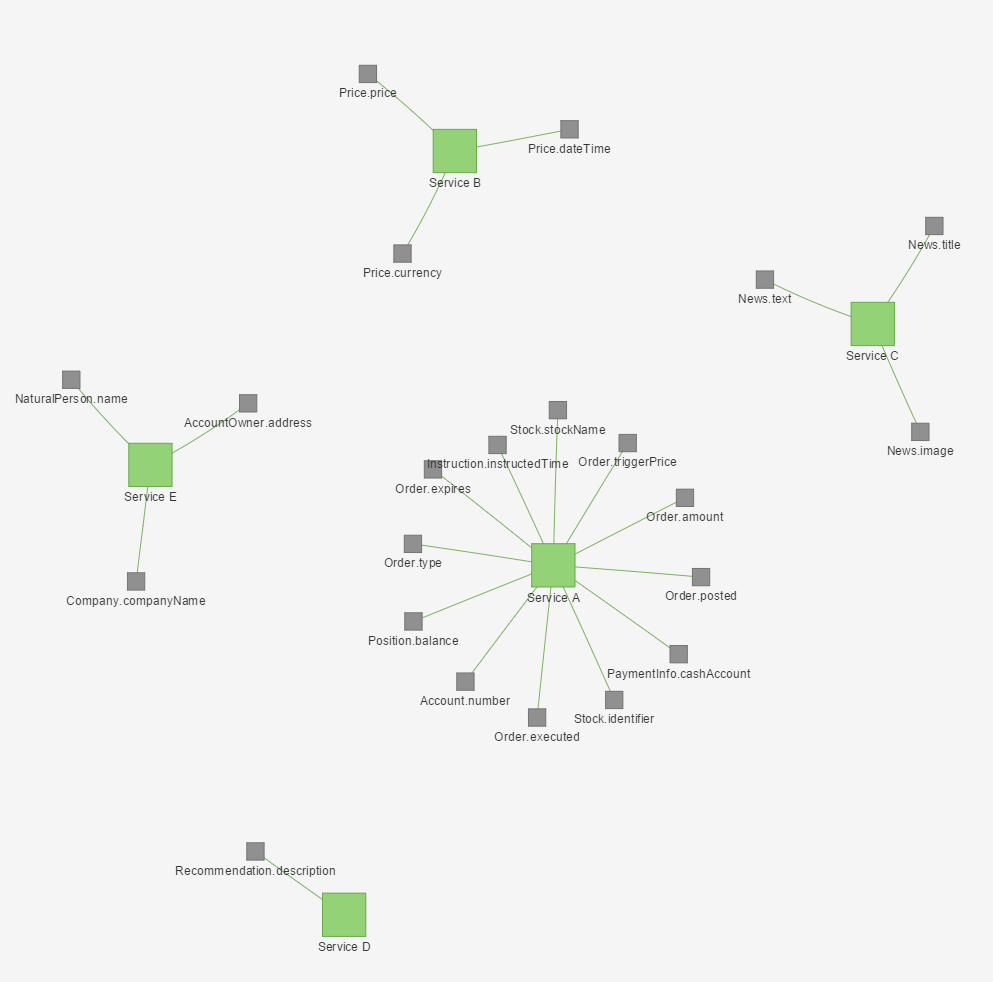
\includegraphics[scale=0.5]{images/trading_service_cut.png}
	\caption{Trading System actual service cuts}
	\label{fig:tradingCutsTool}
\end{figure}

The parameters that produce a cut as seen in \ref{fig:tradingCutsTool} are the following:

\begin{itemize}
\item Coupling criteria priorities: Defaults as defined in \ref{sec:defaultPriorities}
\item Number of services: 5
\end{itemize}

The presented candidate service cuts match exactly the expected services and are therefore considered a good result.

\subsubsection{Priorities Sensitivity}

The candidate service cuts are very stable when changing the priorities. Changing the two relevant cohesiveness parameters \textit{Identity \& Lifecycle Commonality} and \textit{Semantic Proximity} to any combination between \textit{XS} and \textit{L} only affects the result when both set to \textit{L}. With these priorities the Service Cutter suggests an own service for \textit{Stock.stockName} and \textit{Stock.identifier} instead of \textit{Recommendation.description}.

An own service for stocks is reasonable as these nanoentities can be categorized as master data and not transaction data like most of the other nanoentities in the order service. Requesting 6 number of services with these priorities creates cuts for both the recommendation and the stock service. 

Changing the priority of compatibility or constraint criteria to any value between \textit{XS} and \textit{L} does not affect the resulting cuts. However the possibility to request a small number of services gets lost as too many relations between nanoentites are cut if criteria scoring negative values receive a high priority. 

\subsubsection{Number of Services}

As Girvan-Newman receives a number of services parameter we can analyze how a monolithic architecture would be split up step by step. The resulting services by each parameter are listed in Table \ref{tab:tradingNumberOfServices}.

\begin{table}[H]
	\centering
	\caption{Girvan-Newman cuts of trading system with different number of services}
	\label{tab:tradingNumberOfServices}
	\begin{tabular}{|p{60pt}|p{200pt}|}
		\hline	
		\textbf{Number of services} & \textbf{Services}  \\
		\hline
		1 & Monolith \\
		\hline
		2 & Customer Service extracted \\
		\hline
		3 & Price Service extracted  \\
		\hline
		4 & News Service extracted  \\
		\hline
		5 & Recommendation Service extracted  \\
		\hline
		6 & Not supported\\
		\hline
		7 & Payment Service and Instruction Service extracted \\
		\hline
		8 & Stock Service extracted \\
		\hline
		9 & Stock Service splitted in \textit{Stock.name} and \textit{Stock.identifier} \\
		\hline
	\end{tabular}
\end{table}

Reasonable cuts are presented for up to 8 different services. The results produced by Girvan-Newman with the Trading System example are very satisfying as \textit{good} results are presented with almost all combinations of parameters. 

\subsection{Leung Algorithm Assessment}

Leung produces varying suggested cuts as it is not a deterministic algorithm. The algorithm is therefore harder to analyze, as we can't determine if changes in results emerge from changes in priorities or by coincidence. 

Generally speaking the results are similar as those by Girvan-Newman. With the default priorities, the result matches the one of Girvan-Newman shown in Figure \ref{fig:tradingCutsTool} in approximately 50\%. In the cases it is not matching it suggests fewer service by merging two services together. This is due to the label propagation problem described in XXX.
%TODO describe propagation problem in algorithm description. 

\subsubsection{Priorities Sensitivity}

As already mentioned we can't assess the priority sensitivity with Leung. Changing criteria priorities to values from \textit{XS} to \textit{L} has in some cases produced the following results differing from the one shown in Figure \ref{fig:tradingCutsTool}.

\begin{itemize}
	\item An extra service for PaymentInfo.
	\item An extra service for Stock.
	\item An extra service for Account.
	\item A service combining Account, PaymentInfo and Position.
	\item A service combining News and Stock.
\end{itemize}

Except of the last cut we find reasonable justifications for all cases. In fact, combining PaymentInfo, Account and Position into one service seems to be a considerable suggestion we have not thought of before. These entities are closely related to an account while the other entities in the order service are more focused on the trading itself. 

\subsubsection{Number of Services}

The number of services suggested by Leung vary between 2 and 7 services. There is a tendency towards a higher number of services when cohesiveness criteria are prioritized high and compatibility, and constraints criteria are prioritized low. The same applies vice versa. 

With only small changes to the priorities Leung commonly suggests 4 or 5 services which matches with our expectation. %TODO meistens?

\subsection{Conclusion}

In conclusion we can say that the Service Cutter did suggest the Trading System service cuts as we expected. For both algorithms most results can be considered \textit{good} with only one or two exceptions where the result was considered \textit{acceptable}. These are excellent results for a first test of the Service Cutters scoring and algorithms. 

The tests furthermore show the advantages and disadvantages of a deterministic algorithm. Girvan-Newman produced very stable results and nicely shows the path from a monolith to a more service oriented architecture. Leung on the other hand is harder to analyze but provided us more reasonable candidate service cuts we have not considered before. Leung also suggests a reasonable number of services while this consideration completely lies in the responsibility of the user when using Girvan-Newman.

\section{Cargo Tracking System - Domain-Driven Design Sample}
\label{sec:dddSample}

The Cargo Tracking System is a well known software project created to illustrate the concepts and patterns described in the \gls{DDD} book by E. Evans\cite{evans2003domain}. The DDDSample is hosted on Github\cite{dddGithub} and a short screencast on YouTube\cite{dddScreencast} outlines its functionality. 

The Cargo Tracking System provides a domain with a suitable complexity and, unlike the Trading System, comes with a already implemented and well reasoned architecture. With reverse engineering we extracted the domain model, use cases and some characteristics from the code. The Cargo Tracking implements the following functionalities:

\begin{itemize}
	\item The main focus is to transport a \textit{Cargo} from \textit{Location} A to \textit{Location} B. \textit{Cargos} are created with a \textit{TrackingId} and specified with a \textit{RouteSpecification}. Once created, one of multiple suitable \textit{Itinerarys} is assigned.
	\item The system calculates suitable \textit{Itinerarys} for a \textit{Cargo} from existing \textit{Voyages} each containing a list of \textit{CarrierMovements}.
	\item Once a \textit{Cargo} is routed, \textit{HandlingEvents} track the progress of each \textit{Cargo's} \textit{Itinerary}. A \textit{HandlingEvent} contains information about the event and references a \textit{Cargo} on a specific \textit{Voyage} and occurs in a particular \textit{Location}. 
	\item The \textit{Delivery} of a \textit{Cargo} informs about its state, estimated arrival time and contains information whether the \textit{Cargo} is on track or not.
\end{itemize}

The extracted domain model is not a one-to-one copy of the domain classes in the code. The domain classes contain some calculated and therefore redundant information which have been merged into single nanoentities in the domain model shown in Figure \ref{fig:dddSampleAggregates}. 

\begin{figure}[H]
	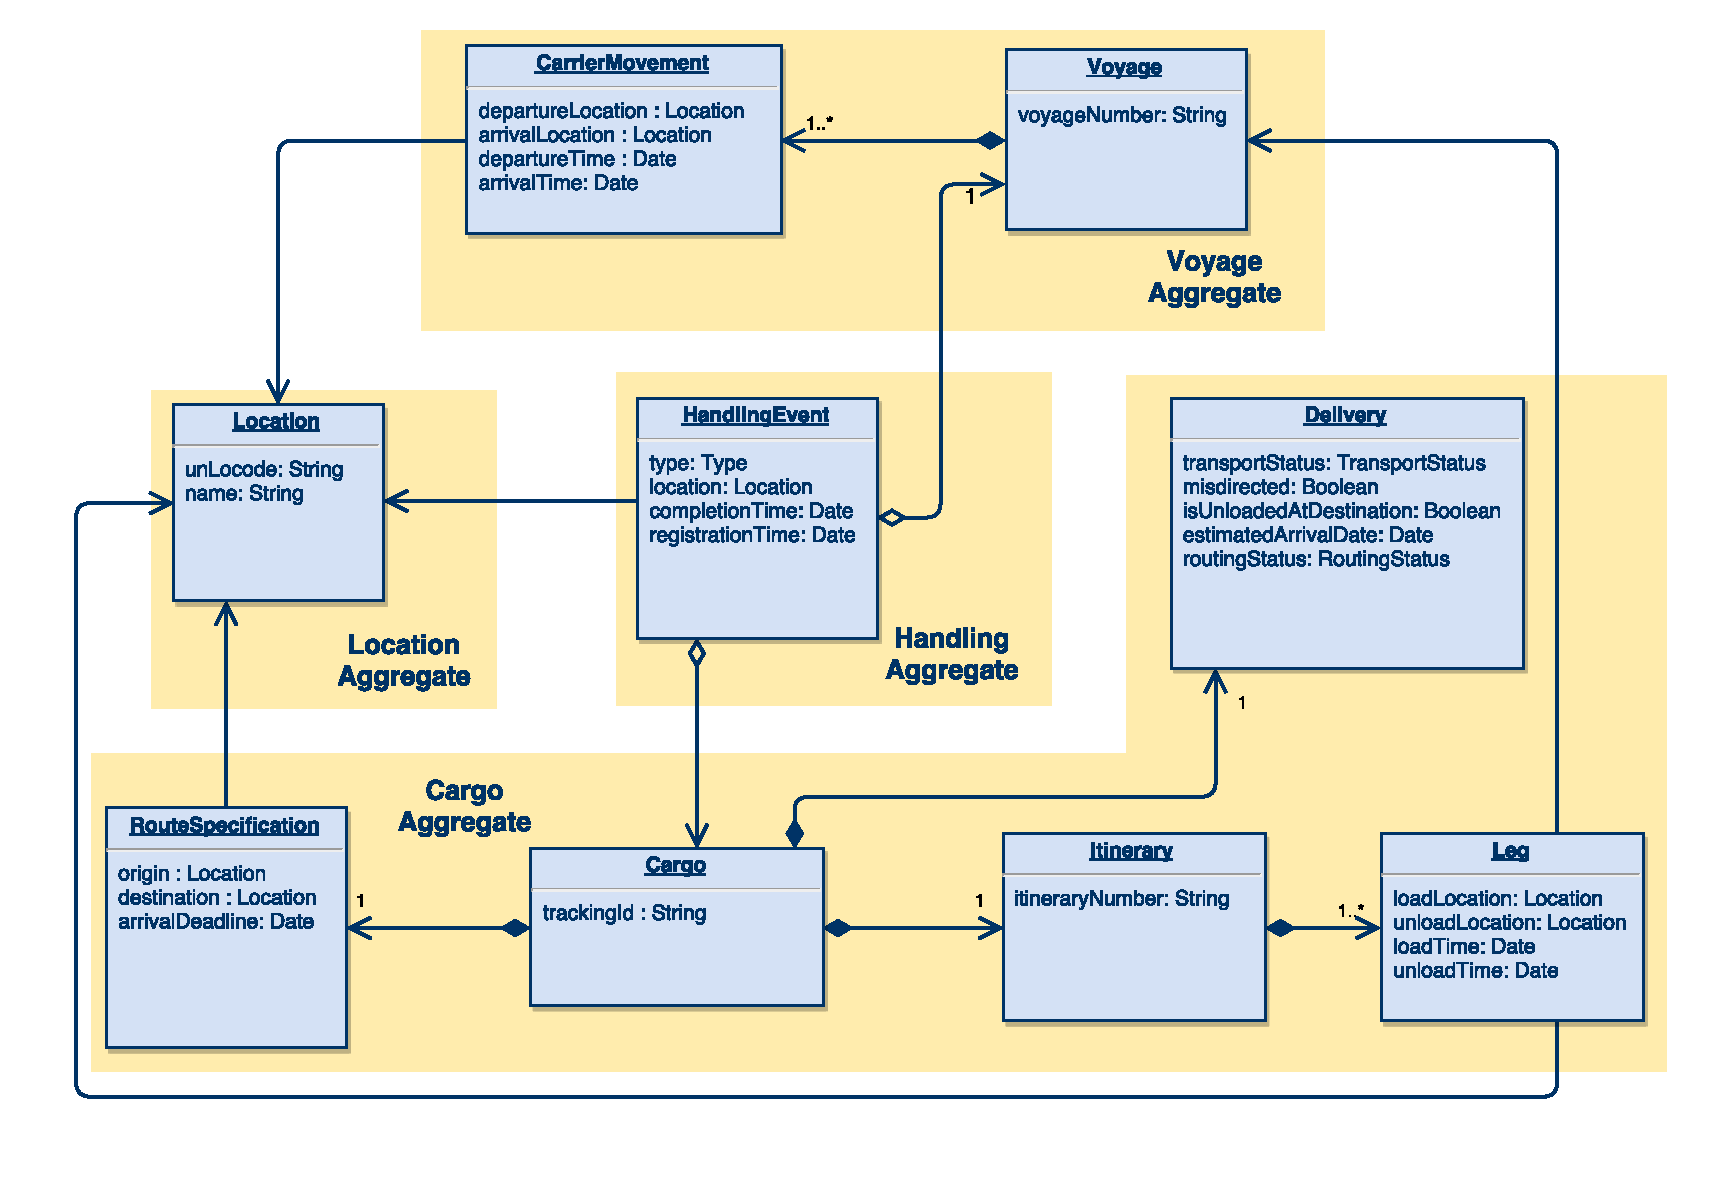
\includegraphics[scale=0.5]{diagrams/ddd_sample_aggregates.pdf}
	\caption{DDD Sample with Aggregates}
	\label{fig:dddSampleAggregates}
\end{figure}

Figure \ref{fig:dddSampleAggregates} additionally outlines the package and aggregate structure provided by the DDDSample which is a first indication about service decomposition. 

The following use cases describe the supported functionality of the application.

\begin{enumerate}
	\item ViewTracking
	\begin{itemize}
		\item Nanoentities written: -
		\item Nanoentities read: Cargo.trackingId, HandlingEvent.type, HandlingEvent.location, HandlingEvent.completionTime, Delivery.transportStatus, Delivery.estimatedArrivalTime, Delivery.misdirected, Voyage.voyageNumber, RouteSpecification.destination, Stock.stockName
	\end{itemize}
	
	\item ViewCargos
	\begin{itemize}
		\item Nanoentities written: -
		\item Nanoentities read: Cargo.trackingId, RouteSpecification.destination, RouteSpecification.arrivalDeadline, Delivery.routingStatus, Itinerary.itineraryNumber
	\end{itemize}
	
	\item BookCargo
	\begin{itemize}
		\item Nanoentities written: Cargo.trackingId, RouteSpecification.origin, RouteSpecification.arrivalDeadline, RouteSpecification.destination
		\item Nanoentities read: Location.unLocode
	\end{itemize}
	
	\item ChangeCargoDestination
	\begin{itemize}
		\item Nanoentities written: RouteSpecification.destination
		\item Nanoentities read: Cargo.trackingId, RouteSpecification.destination
	\end{itemize}
	
	\item RouteCargo
	\begin{itemize}
		\item Nanoentities written: Itinerary.itineraryNumber, Leg.loadLocation, Leg.unloadLocation, Leg.loadTime, Leg.unloadTime
		\item Nanoentities read: Cargo.trackingId, RouteSpecification.destination, RouteSpecification.origin, RouteSpecification.arrivalDeadline, Location.unLocode, Voyage.voyageNumber, CarrierMovement.departureLocation, CarrierMovement.arrivalLocation, CarrierMovement.departureTime, CarrierMovement.arrivalTime
	\end{itemize}
	
	\item Create Location
	\begin{itemize}
		\item Nanoentities written: Location.unLocode, Location.name
		\item Nanoentities read: -
	\end{itemize}

	\item Create Voyage
	\begin{itemize}
		\item Nanoentities written: Voyage.voyageNumber
		\item Nanoentities read: -
	\end{itemize}
	
	\item Add CarrierMovement
	\begin{itemize}
		\item Nanoentities written: CarrierMovement.departureLocation, CarrierMovement.arrivalLocation, CarrierMovement.departureTime, CarrierMovement.arrivalTime
		\item Nanoentities read: Voyage.voyageNumber
	\end{itemize}
	
	\item Handle Cargo Event
	\begin{itemize}
		\item Nanoentities written: HandlingEvent.type, HandlingEvent.completionTime, HandlingEvent.registrationTime, HandlingEvent.location, Delivery.transportStatus, Delivery.misdirected, Delivery.estimatedArrivalTime, Delivery.isUnloadedAtDestination, Delivery.routingStatus
		\item Nanoentities read: Voyage.voyageNumber, Cargo.trackingId
	\end{itemize}
\end{enumerate}

In addition to the use cases, we identified the following characteristics.

\textbf{Volatility}

\begin{itemize}
	\item \textbf{Often}: HandlingEvent.type, HandlingEvent.completionTime, HandlingEvent.registrationTime, HandlingEvent.location, Delivery.transportStatus 
	\item \textbf{Rarely}: Location.unLocode, Location.name
\end{itemize} 

\textbf{Change Similarity}

\begin{itemize}
	\item \textbf{Rarely}: Location.unLocode, Location.name
\end{itemize}

Furthermore all default characteristics as documented in Section \ref{sec:couplingCriteria} are taken into account.

The DDDSample provides multiple interfaces depending on the user's role. The main interface provides tracking information, the administration panel offers means to create cargos and plan their itinerary and an additional interface is used to inform about handling events. Out of these distinction by the \gls{UI} we defined responsibility areas listed in Table \ref{tab:dddResponsibilites} each containing a group of nanoentities a user role is responsible for.

\begin{table}[H]
	\centering
	\caption{Responsibility Areas in DDDSample}
	\label{tab:dddResponsibilites}
	\begin{tabular}{|p{90pt}|p{200pt}|}
		\hline	
		\textbf{Responsibility Area} & \textbf{Nanoentities}  \\
		\hline
		Cargoplaner & Cargo.trackingId \newline RouteSpecification.origin\newline RouteSpecification.destination\newline RouteSpecification.arrivalDeadline\newline Itinerary.itineraryNumber\newline Leg.loadLocation\newline Leg.unloadLocation\newline Leg.loadTime\newline Leg.unloadTime\newline Delivery.estimatedArrivalTime\newline Delivery.routingStatus  \\
		\hline
		CargoTracker & HandlingEvent.type\newline HandlingEvent.completionTime\newline HandlingEvent.registrationTime\newline HandlingEvent.location\newline Delivery.transportStatus\newline Delivery.misdirected\newline Delivery.isUnloadedAtDestination  \\
		\hline
		VoyageManager & Voyage.voyageNumber\newline CarrierMovement.departureLocation\newline CarrierMovement.arrivalLocation\newline CarrierMovement.departureTime\newline CarrierMovement.arrivalTime \\
		\hline
		Admin & Location.name, Location.unLocode \\
		\hline
	\end{tabular}
\end{table}

\subsection{Expected Service Cuts}

From our experience in software architecture we expect the Service Cutter to decompose the Cargo Tracking System into the services presented in Figure \ref{fig:dddSampleServices}.

\begin{figure}[H]
	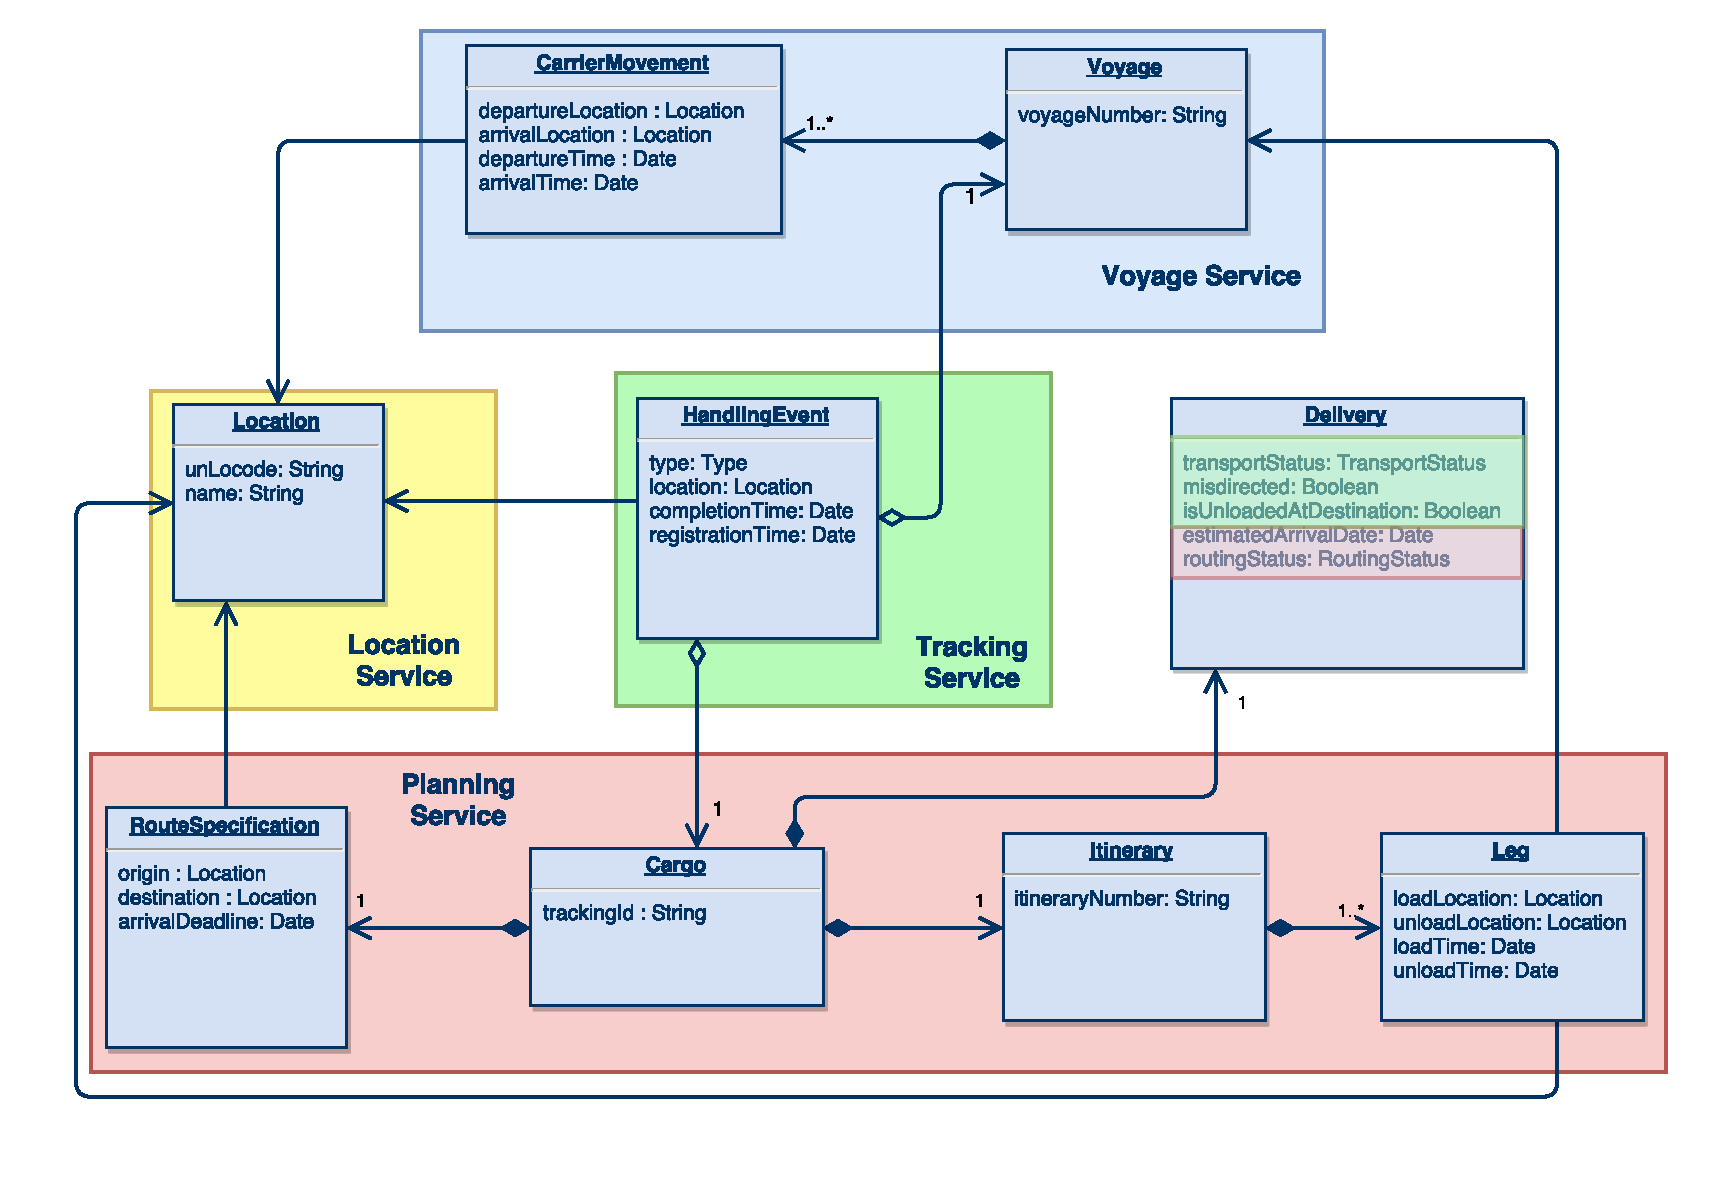
\includegraphics[scale=0.5]{diagrams/ddd_sample_services.pdf}
	\caption{DDD Sample with expected services}
	\label{fig:dddSampleServices}
\end{figure}

As there are not many compatibility criteria defined, the main reasons for our decomposition solution are responsibilities and semantic proximity by use cases:

\begin{itemize}
	\item The \textit{Voyage Service} contains all nanoentities regarding actual voyages and their movements, regardless of any cargo. 
	\item The \textit{Location Service} is separated as a consequence of the low volatility and change similarity of these nanoentities. Locations are used and referred from almost all entities but very rarely written. This service could be categorized as a master data service.
	\item The \textit{Planning Service} handles all nanoentities regarding cargos and their itinerary. 
	\item The \textit{Tracking Service} is responsible to track the actual events of a cargo. The aggregates defined in the DDDSample assign the delivery to the Planning Service. In our opinion the nanoentities \textit{transportStatus}, \textit{misdirected} and \textit{isUnloadedAtLocation} are better assigned to the Tracking Service as they are defined as a consequence of handling events.
\end{itemize}

\subsection{Girvan-Newman Algorithm Assessemnt}

For the Cargo Tracking System the default priorities were adjusted to the following values:

\begin{itemize}
	\item Volatility: \textit{S} instead of \textit{XS}
	\item Change Similarity: \textit{S} instead of \textit{XS}
	\item Responsibility: \textit{L} instead of \textit{M}
\end{itemize}

The resulting candidate service cuts by the Girvan-Newman algorithm for 4 services are shown in Figure \ref{fig:dddGirvanNewman}.

\begin{figure}[H]
	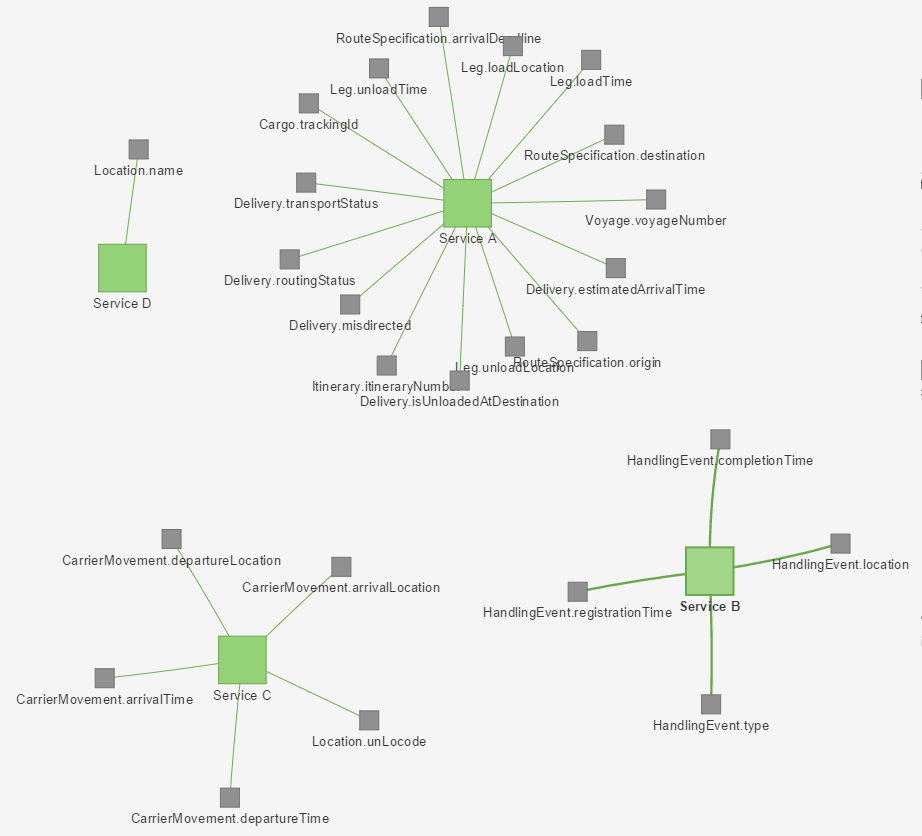
\includegraphics[scale=0.7]{images/ddd_girvan_4.png}
	\caption{Cargo Tracking System Service Cuts by Girvan-Newman}
	\label{fig:dddGirvanNewman}
\end{figure}

Surprisingly, the location has been split to Service D and Service C. Service C contains the carrierMovement nanoentities but misses the voyageNumber which is closely related to the carrierMovement through responsibilities and use cases. Service B represents the handling aggregate as defined by the DDDSample but does not contain delivery nanoentites as expected by us. 

None of the service contains the nanoentities as expected by us and only Service B can be categorized as reasonable service cut. We rate this a \textit{bad} result. 

The split of location might be due to the fact that in most use cases only Location.unLocode is used and not Location.name. We changed the priority for \textit{Semantic Proximity} from \textit{M} to \textit{S} which resulted in the candidate service cuts shown in Figure \ref{fig:dddGirvanNewmanS}

\begin{figure}[H]
	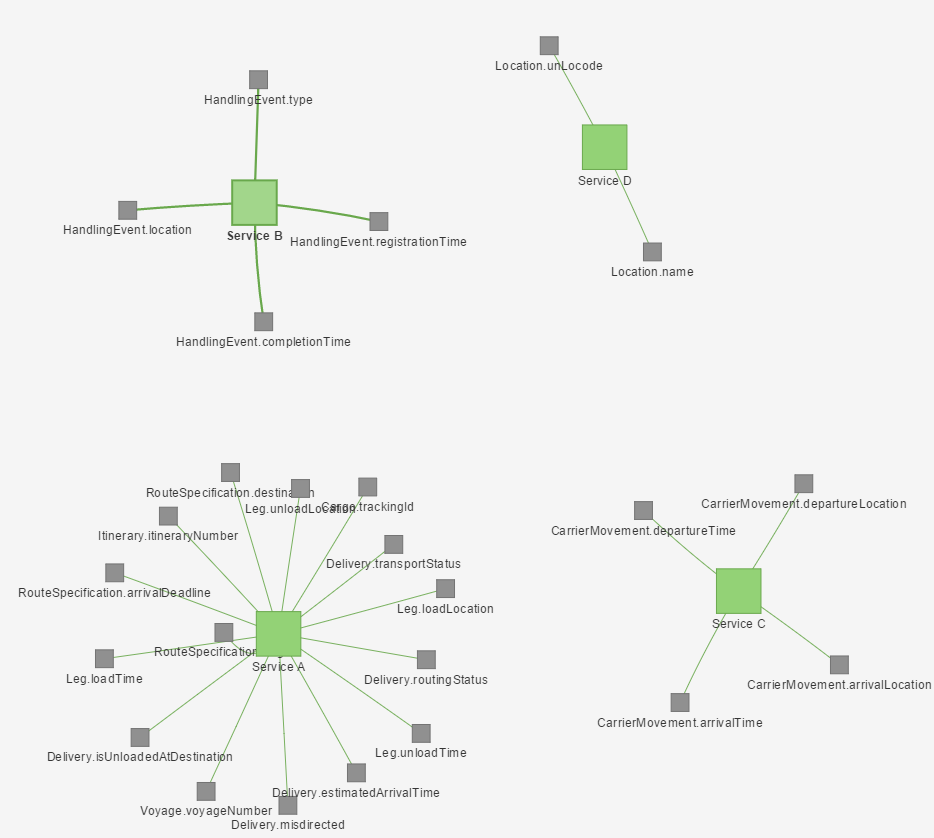
\includegraphics[scale=0.7]{images/ddd_girvan_4_proximity_s.png}
	\caption{Semantic Proximity with Priority S instead of M}
	\label{fig:dddGirvanNewmanS}
\end{figure}

Location has now an own service as expected. This improves the result a little but still not enough to consider it \textit{acceptable}.

\subsubsection{Priorities Sensitivity}

Changing priorities of the relevant coupling criteria to values between \textit{XS} and \textit{L} results in minor changes. The following alternations have been produced:

\begin{itemize}
	\item Delivery.transportStatus is assigned to the service containing handling events if \textit{Identity \&Lifecycle Commonality} is set to \textit{XS}. This is closer to our expectation of a tracking service.
	\item Increasing the priority of \textit{Semantic Proximity} to \textit{L} produces an unreasonable service containing Cargo, Voyage and RouteSpecification nanoentities.
\end{itemize}

We were not able to produce \textit{acceptable} or \textit{good} results for the Cargo Tracking System with Girvan-Newman. The sensitivity of the results on priority changes seems acceptable. 

\subsection{Leung Algorithm Assessment}

Like Girvan-Newman, the Leung algorithm only suggests a location service if \textit{Semantic Proximity} is set to \textit{S} instead of \textit{M}. The candidate service cuts are shown in Figure \ref{fig:dddleungVoyage}.	

\begin{figure}[H]
	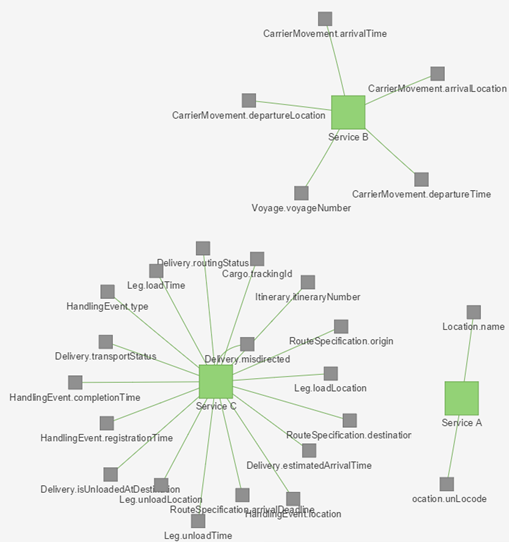
\includegraphics[scale=0.9]{images/leung_voyage.png}
	\caption{Cargo Tracking System Service Cuts by Leung}
	\label{fig:dddleungVoyage}
\end{figure}

A location and a voyage service have been extracted while the planning and tracking service are merged together. A different run with the same priorities is shown in Figure \ref{fig:dddleungTracking}.

\begin{figure}[H]
	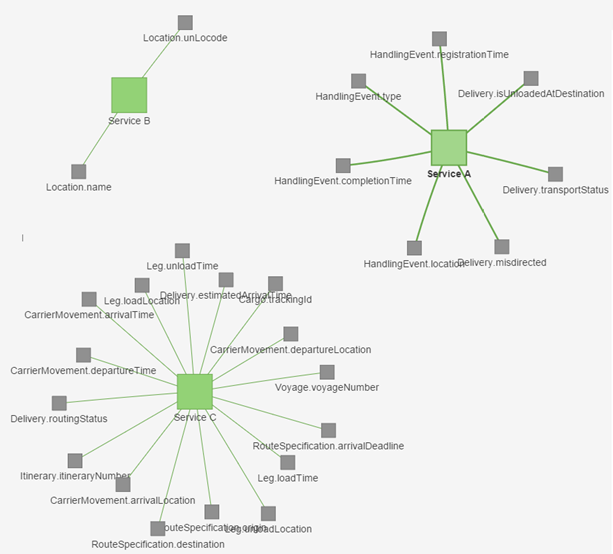
\includegraphics[scale=0.9]{images/leung_tracking.png}
	\caption{Cargo Tracking System Service Cuts by Leung}
	\label{fig:dddleungTracking}
\end{figure}

This time Leung extracted the tracking service and kept voyage and planning services together. Noteworthy is the fact that Leung splits the delivery entity in two different services the same way we expected it. 

Other runs resulted in similar cuts whereas often only the location service was extracted. The cuts done by Leung meet our expectations precisely but provides less services than expected. We assume this results from the label propagation problem described in Section XX. 
%TODO: describe Leung problem. 

The results provided by Leung can be classified as \textit{acceptable}.









